\documentclass[utf8x, 12pt]{G7-32} 
\sloppy

% Настройки стиля ГОСТ 7-32
% Для начала определяем, хотим мы или нет, чтобы рисунки и таблицы нумеровались в пределах раздела, или нам нужна сквозная нумерация.

%\EqInChapter % формулы будут нумероваться в пределах раздела
%\TableInChapter % таблицы будут нумероваться в пределах раздела
%\PicInChapter % рисунки будут нумероваться в пределах раздела

% Добавляем гипертекстовое оглавление в PDF
\usepackage[
bookmarks=true, colorlinks=true, unicode=true,
urlcolor=black,linkcolor=black, anchorcolor=black,
citecolor=black, menucolor=black, filecolor=black,
]{hyperref}

% Изменение начертания шрифта --- после чего выглядит таймсоподобно.
% apt-get install scalable-cyrfonts-tex

\IfFileExists{cyrtimes.sty}
    {
        \usepackage{cyrtimespatched}
    }
    {
        % А если Times нету, то будет CM...
    }

\usepackage{graphicx}   % Пакет для включения рисунков
\DeclareGraphicsExtensions{.jpg,.pdf,.png}
% С такими оно полями оно работает по-умолчанию:
% \RequirePackage[left=20mm,right=10mm,top=20mm,bottom=20mm,headsep=0pt]{geometry}
% Если вас тошнит от поля в 10мм --- увеличивайте до 20-ти, ну и про переплёт не забывайте:
\geometry{right=20mm}
\geometry{left=30mm}



% Произвольная нумерация списков.
\usepackage{enumerate}

\setcounter{tocdepth}{3} %Подробность оглавления
%4 это chapter, section, subsection, subsubsection и paragraph
%3 это chapter, section, subsection и subsubsection
%2 это chapter, section, и subsection
%1 это chapter и section
%0 это chapter.



\begin{document}

\frontmatter 
\begin{center} 

\large САНКТ-ПЕТЕРБУРГСИЙ ГОСУДАРСТВЕННЫЙ ПОЛИТЕХНИЧЕСКИЙ УНИВЕРСИТЕТ

\large Кафедра Компьютерных Систем и Программных Технологий \\[4.5cm] 

\huge ОТЧЕТ \\[0.6cm] % название работы, затем отступ 0,6см
\large по лабораторной работе №1\\
\large Тема: <<Основные виды анализа аналоговых электронных устройств в среде проектирования Cadence Allegro>>\\
\large Дисциплина: <<Автоматическое проектирование аналоговых цифровых устройств>>\\[2.7cm]

\end{center} 

\begin{flushright}
Выполнили: студенты гр. 53501/2 \\
Пономарев М.A \\
Федоров Е.М \\[1.2cm]

Преподаватель \\
Балтруков Н.Н
\end{flushright}


\vfill 

\begin{center} 
\large Санкт-Петербург \\
2015
\end{center} 

\thispagestyle{empty}

\thispagestyle{empty}
\setcounter{page}{0}
\tableofcontents
\clearpage
\mainmatter



\chapter{Задание}

\begin{itemize}
	\item На языке Verilog описать представленную ниже схему
	
\begin{figure}[h]
	\begin{center}
		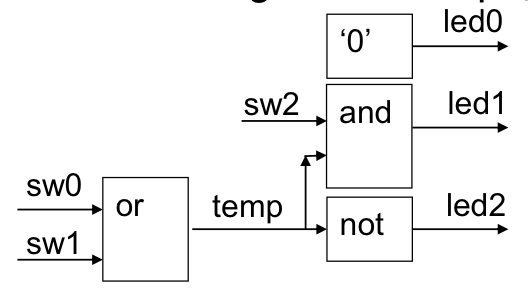
\includegraphics[width=7cm]{img/shema}
	\end{center}
	\vspace{-5mm}\caption{Схема устройства}
\end{figure}	
	
	\item Посмотреть синтезированную пакетом QII схему (RTL Viewer)
	\item Осуществить функциональное моделирование 
	\item Назначить выводы СБИС
	\item Осуществить полную компиляцию, программирование платы и проверить работу проекта на плате 
\end{itemize}

\chapter{Решение}

Для определения логики работы файла создадим Verilog HDL файл. В результате получаем следующий код:

\begin{figure}[hhh!]
	\begin{center}
		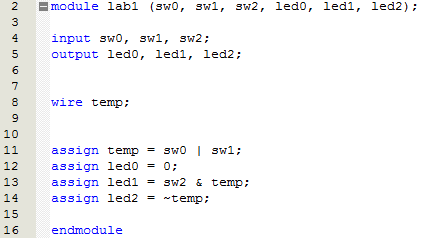
\includegraphics[width=12cm]{img/vhdl}
	\end{center}
	\vspace{-5mm}\caption{VHDL код}
\end{figure}


Для просмотра логической схемы работы устройства воспользуемся RTL Viewer. В результате получаем:

\begin{figure}[hhh!]
	\begin{center}
		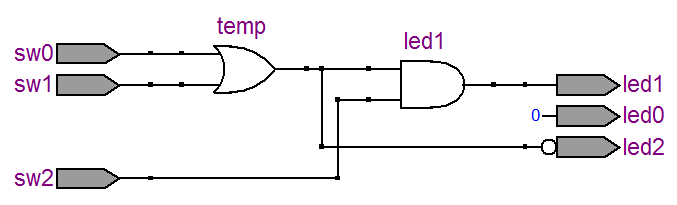
\includegraphics[width=12cm]{img/RTL_Viewer}
	\end{center}
	\vspace{-5mm}\caption{Логическая схема устройства}
\end{figure}


Осуществим функциональное моделирование. Для этого создадим Vector Waveform File, определим значение входных сигналов. Запустим функциональное моделирование, получим:

\begin{figure}[hhh!]
	\begin{center}
		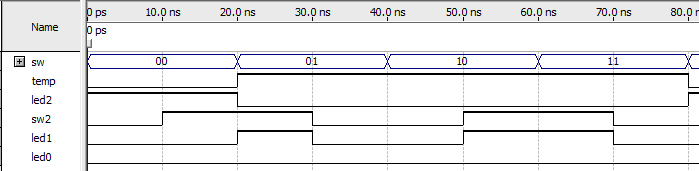
\includegraphics[width=12cm]{img/waveform}
	\end{center}
	\vspace{-5mm}\caption{Векторная диаграмма}
\end{figure}


\chapter{Выводы}

В ходе выполнения лаобораторной работы было спроектировано устройство на языке Verilog HDL, осуществлено функциональное моделировние для проверки правильности работы и проверка работы устройстройства на плате.


\end{document}
